
\documentclass{beamer}
\usetheme{ucl}

\usepackage[utf8]{inputenc}


%%% Increase the height of the banner: the argument is a scale factor >=1.0
%\setbeamertemplate{banner}[ucl][10.0]

%%% Change the colour of the main banner
%%% The background should be one of the UCL colours (except pink or white):
%%%   black,darkpurple,darkred,darkblue,darkgreen,darkbrown,richred,midred,
%%%   navyblue,midgreen,darkgrey,orange,brightblue,brightgreen,lightgrey,
%%%   lightpurple,yellow,lightblue,lightgreen,stone
\setbeamercolor{banner}{bg=darkpurple}
%\setbeamercolor{banner}{bg=yellow,fg=black}

%%% Add a stripe behind the banner
%\setbeamercolor{banner stripe}{bg=darkpurple,fg=black}

%%% The main structural elements
\setbeamercolor{structure}{fg=black}

%%% Author/Title/Date and slide number in the footline
\setbeamertemplate{footline}[author title date]

%%% Puts the section/subsection in the headline
% \setbeamertemplate{headline}[section]

%%% Puts a navigation bar on top of the banner
%%% For this to work correctly, the each \section command needs to be
%%% followed by a \subsection. Requires one extra compile.
% \setbeamertemplate{headline}[miniframes]
%%% Accepts an optional argument determining the width
% \setbeamertemplate{headline}[miniframes][0.3\paperwidth]


%%% Puts the frame title in the banner
%%% Won't work correctly with the above headline templates
%\useoutertheme{ucltitlebanner}
%%% Similar to above, but smaller (and puts subtitle on same line as title)
\useoutertheme[small]{ucltitlebanner}

%%% Gives block elements (theorems, examples) a border
% \useinnertheme{blockborder}
%%% Sets the body of block elements to be clear
% \setbeamercolor{block body}{bg=white,fg=black}

%%% Include CSML logo on title slide
%\titlegraphic{\includegraphics[width=0.16\paperwidth]{csml_logo}}

%%% Include CSML logo in bottom right corner of all slides
%\logo{\includegraphics[width=0.12\paperwidth]{csml_logo}}

%%% Set a background colour
% \setbeamercolor{background canvas}{bg=lightgrey}

%%% Set a background image
%%% Some sample images are available from the UCL image store:
%%%   https://www.imagestore.ucl.ac.uk/home/start
% \setbeamertemplate{background canvas}{%
%   \includegraphics[width=\paperwidth]{imagename}}



%%%%%% Some other settings that can make things look nicer
%%% Set a smaller indent for description environment
\setbeamersize{description width=2em}
%%% Remove nav symbols (and shift any logo down to corner)
\setbeamertemplate{navigation symbols}{\vspace{-2ex}}








\DeclareMathOperator{\Cov}{Cov}
\DeclareMathOperator{\Var}{Var}
\DeclareMathOperator{\E}{\mathbb{E}}
\DeclareMathOperator{\Proba}{\mathbb{P}}

\newcommand{\Covb}[2]{\ensuremath{\Cov\!\left[#1,#2\right]}}
\newcommand{\Eb}[1]{\ensuremath{\E\!\left[#1\right]}}
\newcommand{\Pb}[1]{\ensuremath{\Proba\!\left[#1\right]}}
\newcommand{\Varb}[1]{\ensuremath{\Var\!\left[#1\right]}}

% norm
\newcommand{\norm}[1]{\| #1 \|}

\newcommand{\indep}{\rotatebox[origin=c]{90}{$\models$}}





\usepackage{mathptmx,amsmath,amssymb,graphicx,bibentry,bbm,ragged2e}
\usepackage[english]{babel}

\makeatletter

\newcommand{\noun}[1]{\textsc{#1}}
\newcommand{\jitem}[1]{\item \begin{justify} #1 \end{justify} \vfill{}}
\newcommand{\sframe}[2]{\frame{\frametitle{#1} #2}}

\newenvironment{centercolumns}{\begin{columns}[c]}{\end{columns}}
%\newenvironment{jitem}{\begin{justify}\begin{itemize}}{\end{itemize}\end{justify}}



%\usetheme{Warsaw}
%\setbeamertemplate{footline}[text line]{}
%\setbeamertemplate{headline}{}
%\setbeamercolor{structure}{fg=purple!50!blue, bg=purple!50!blue}

%\setbeamersize{text margin left=15pt,text margin right=15pt}

%\setbeamercovered{transparent}


\@ifundefined{showcaptionsetup}{}{%
 \PassOptionsToPackage{caption=false}{subfig}}
\usepackage{subfig}

\usepackage[utf8]{inputenc}
\usepackage[T1]{fontenc}

\usepackage{multirow}


\makeatother

\def \draft {1}

\usepackage{xparse}
\usepackage{ifthen}
\DeclareDocumentCommand{\comment}{m o o o o}
{\ifthenelse{\draft=1}{
    \textcolor{red}{\textbf{C : }#1}
    \IfValueT{#2}{\textcolor{blue}{\textbf{A1 : }#2}}
    \IfValueT{#3}{\textcolor{ForestGreen}{\textbf{A2 : }#3}}
    \IfValueT{#4}{\textcolor{red!50!blue}{\textbf{A3 : }#4}}
    \IfValueT{#5}{\textcolor{Aquamarine}{\textbf{A4 : }#5}}
 }{}
}
\newcommand{\todo}[1]{
\ifthenelse{\draft=1}{\textcolor{red!50!blue}{\textbf{TODO : \textit{#1}}}}{}
}




\begin{document}

\title
[Modular urban transportation models]{Building and validating modular urban transportation models using scientific workflow systems}
\author[Raimbault]{J.~Raimbault$^{1,2,3}$ and M.~Batty$^{1}$\\\medskip
$^{\ast}$\texttt{j.raimbault@ucl.ac.uk}
}

\institute[UCL]{$^{1}$Center for Advanced Spatial Analysis, University College London\\
$^{2}$UPS CNRS 3611 Complex Systems Institute Paris\\
$^{3}$UMR CNRS 8504 G{\'e}ographie-cit{\'e}s
}




\date[28/01/2021]{Applied Urban Modeling 2021\\
Session 8: Modelling method (2)\\
January 28th, 2021\\
}

\frame{\maketitle}


% Headline summary (50-100 words)
%Large scale urban transportation models such as four-step models require the integration of heteroge- nous data and the coupling of sub-models which can already be consequent in terms of complexity. Therefore, such integrated models are difficult to transfer, reproduce, and validate. We propose a modular and reproducible approach based on scientific workflow systems to build and validate such models. We illustrate it by coupling different open-source components within workflows to construct a four-step transportation model applied to all functional urban areas in the UK, and discuss its application to health indicators within public transport in the context of the COVID-19 crisis.

%  


\section{Introduction}


%Urban transportation models such as four-step models, and more generally land-use transport inter- action models, require the integration of heterogenous data and the coupling of various submodules with possibly high levels of complexity.  

\sframe{Urban transportation models}{

\textit{MATSim model: heterogenous data and integration of many sub-models}

\medskip

\begin{center}
	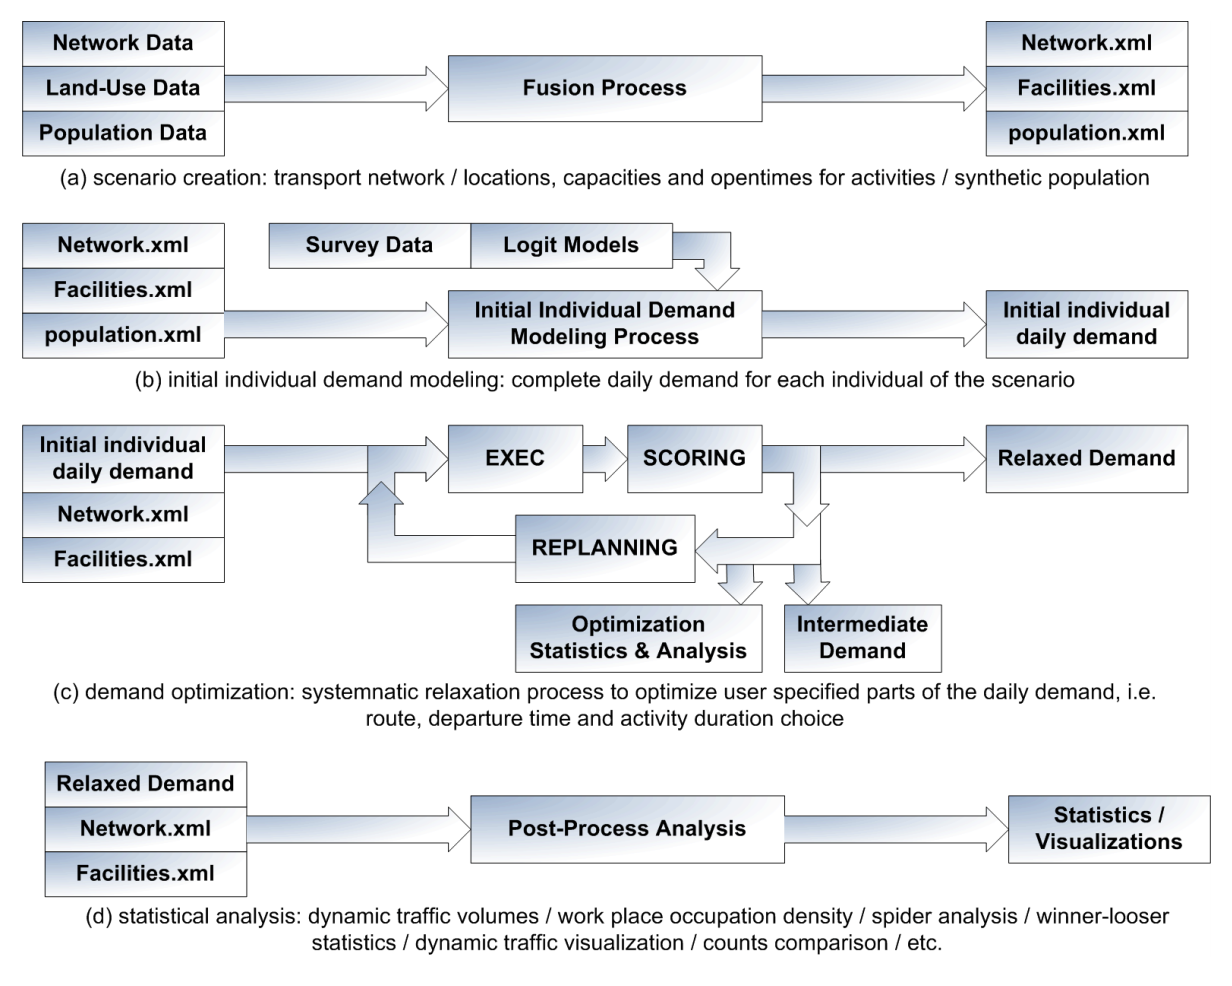
\includegraphics[height=0.7\textheight]{figures/matsim.png}	
\end{center}

Source: \cite{balmer2009matsim}

}

\sframe{Land-use transport models}{

\textit{Land-use transport models as a progressive complexification through coupling of detailed sub-models}

\medskip

\begin{center}
	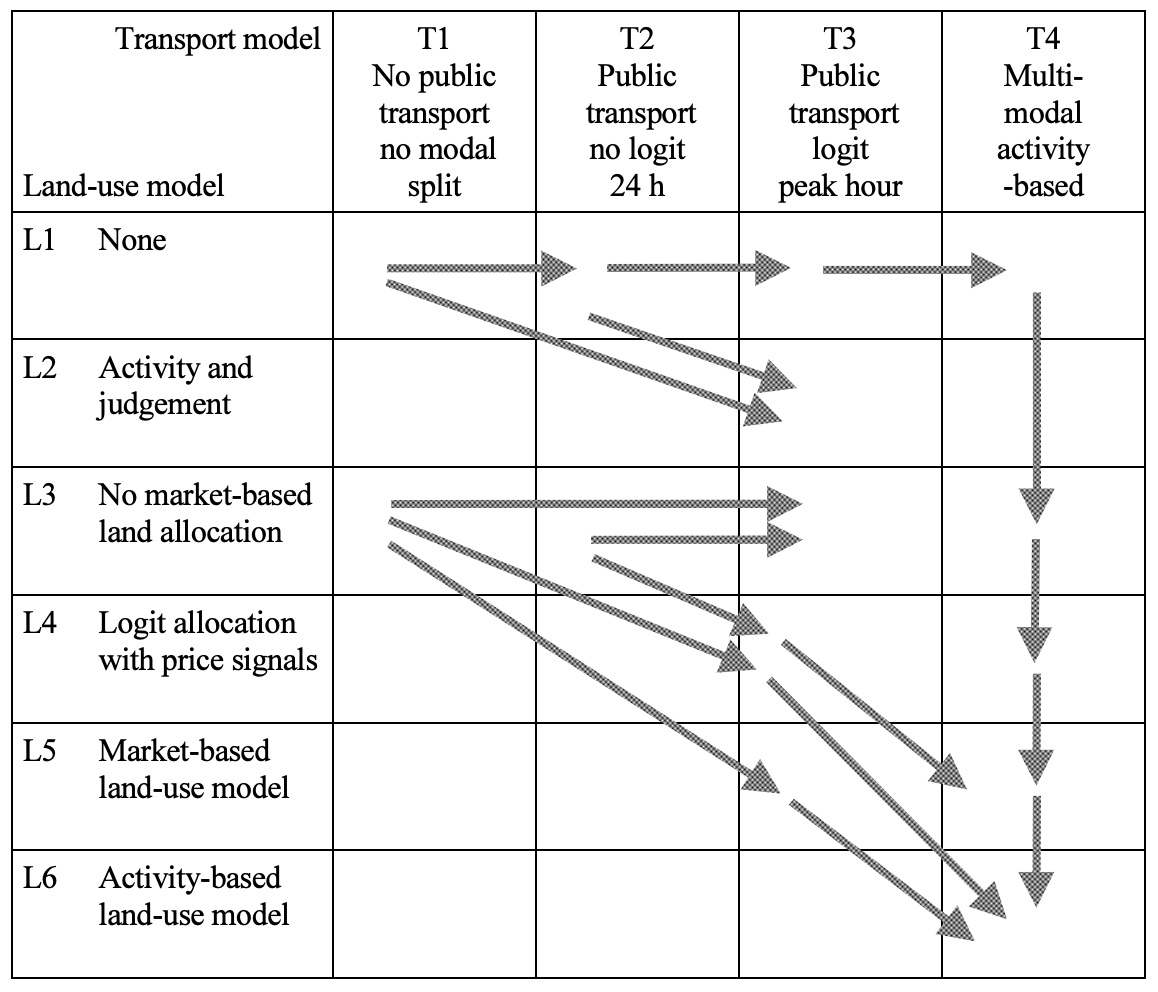
\includegraphics[width=0.45\linewidth]{figures/wegener1.png}\hspace{0.3cm}
	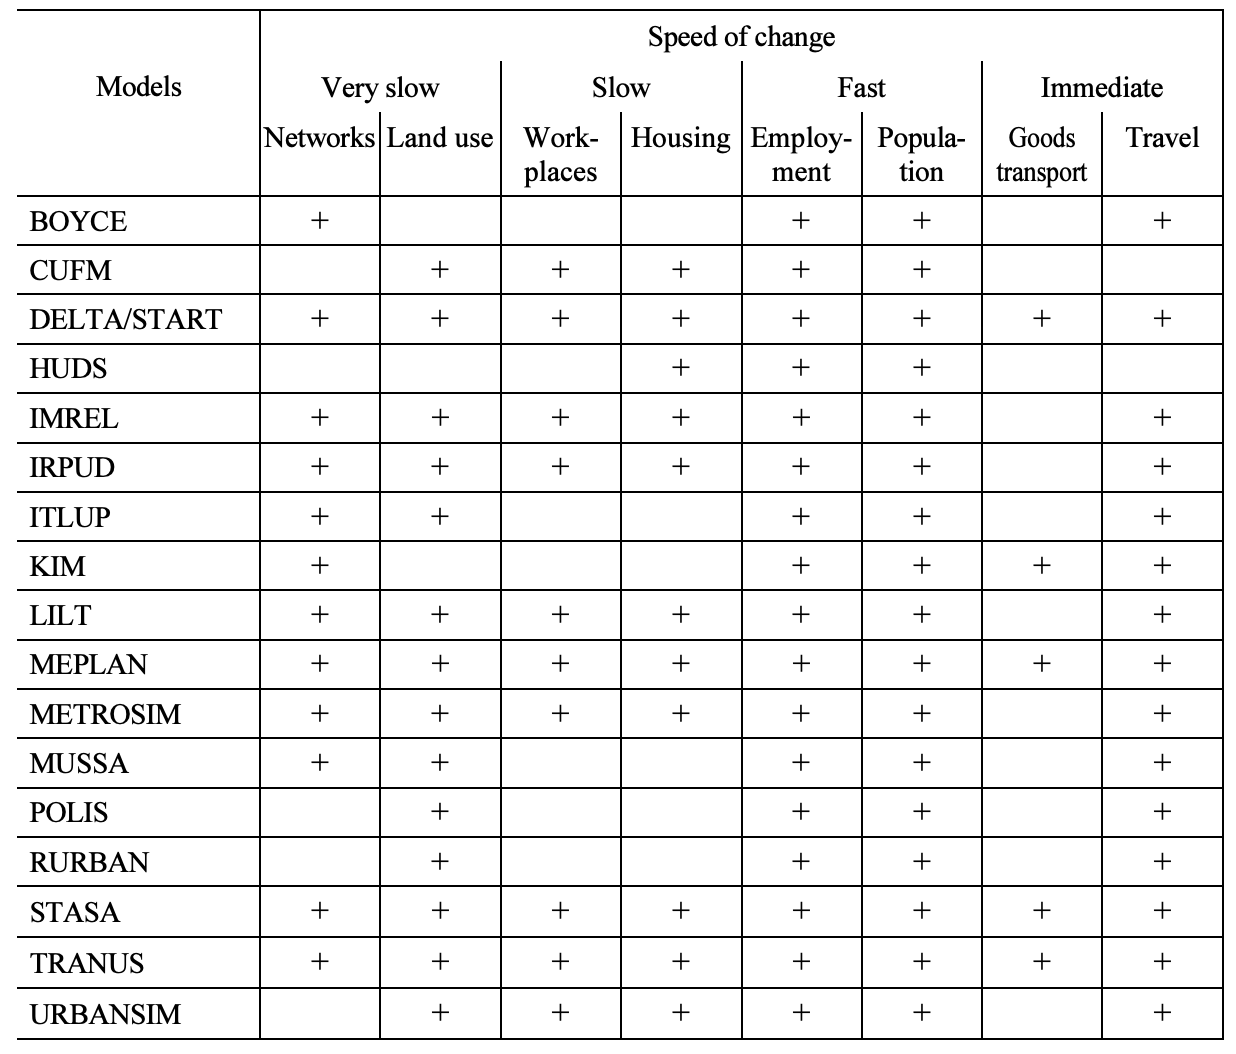
\includegraphics[width=0.45\linewidth]{figures/wegener2.png}
\end{center}

Source: \cite{wegener2004land}

}

\sframe{Relevance of large scale models}{

\textit{Large scale urban models are intrinsically flawed and do not reach their goals of long-term application to planning}: \textbf{Requiem for large scale models in 1973} \cite{lee1973requiem}

\bigskip


\textit{Urban analytics and Smart Cities approaches may follow the same path if they ignore the past and the complexity of cities} \cite{batty2014can}


\bigskip


To foster relevance of large urban models:

\begin{itemize}
	\item Transparency on data and implementation, reproducibility
	\item Validation of models and sub-models: from small simple models well validated to larger integrated models
\end{itemize}

\medskip

$\rightarrow$ Open, reproducible urban models can be shared, coupled into modular integrated models, tested and validated \cite{banos2013pour}



}


\sframe{Towards modular models using workflow systems}{

%This raises issues on the one hand for their implementation, transferability and reproducibility, and on the other hand for their validation which requires large scale numerical experiments to validate the submodules and the whole models.
% This work proposes to tackle both issues by leveraging modularity and transparency for the construction of large urban models in a modular way, using scientific workflow systems to couple the different components of models and to launch numerical experiments for their validation.

% advantages of modularity
%  - generic application to any urban area

% Scientific workflow systems

\textbf{Scientific workflow systems}

\cite{yu2005taxonomy} \cite{barker2007scientific}

\medskip

$\rightarrow$ Execution of numerical experiments and data processing in a systematic, reproducible and domain-specific way

$\rightarrow$ Often coupled to High Performance Computing infrastructures

$\rightarrow$ Flexibility with scripting languages and easier collaboration

\bigskip

\textbf{Proposed approach}

\textit{Build modular urban transportation models from the bottom-up using workflow systems, open source sub-models and open data}

\medskip

$\rightarrow$ Sub-models coupled into the workflow, can be easily replaced

$\rightarrow$ Reproducibility and transparency

$\rightarrow$ Easier transferability of model application

$\rightarrow$ Application of model validation methods


}


\section{Matsim}

% More particularly, we demonstrate this approach by building a modular four-step multimodal trans- portation model using only open-source projects. We couple together the MATSim model (MATSim Community) to simulate the transportation system, the SPENSER model (University of Leeds) for the generation of synthetic population, the QUANT model (University College London) to estimate spatial interactions, and the spatialdata library (OpenMOLE Community) for data preparation. The model is integrated into the DAFNI facility (https://dafni.ac.uk/) which provides a scientific work- flow system for model integration and coupling, direct access to relevant open datasets, visualisation functionalities, and access to a High Performance Computing infrastructure.


\sframe{Case study: integrated models}{



\textbf{Case study:} \textit{Construct a modular four-step multimodal transportation model using open source projects and data}

\bigskip

\textbf{Integrated models:}

\begin{itemize}
	\item MATSim model (MATSim Community) for the transportation system \url{https://www.matsim.org/} \cite{horni2016multi}
	\item SPENSER model (University of Leeds) for the synthetic population \url{https://github.com/nismod/microsimulation}
	\item QUANT model (CASA, University College London) for spatial interactions to generate home-work plans \url{http://quant.casa.ucl.ac.uk/} \cite{milton2019accelerating}
	\item spatialdata library (OpenMOLE community) for data processing \url{https://github.com/openmole/spatialdata} \cite{raimbault2020scala}
\end{itemize}



}

\sframe{Case study: data and implementation}{


\textbf{Data:}

Generic for any Functional Urban Area (GHSL \cite{florczyk2019ghsl}) in the UK: NOMIS census, OrdnanceSurvey roads

\medskip

\textbf{Workflow systems:}

\begin{itemize}
	\item DAFNI facility funded by UKCRIC \url{https://dafni.ac.uk}
	\item OpenMOLE software \url{https://openmole.org/} \cite{reuillon2013openmole}
\end{itemize}

\medskip

\textbf{Implementation}

\begin{itemize}
	\item Currently integrated: synthetic SPENSER population with uniform job locations; simple home-work commuting plans; network and plans prepared into MATSim xml files and fed into a one-mode MATSim.
	\item Work in progress: use the QUANT model to generate more realistic home-work flows.
\end{itemize}



}


%\sframe{Model coupling structure}{
%}


\sframe{DAFNI facility}{

\textit{Platform developed for infrastructure research, providing dataset sharing, model upload, High-performance computing, workflow system.}

\url{https://dafni.ac.uk}

\medskip

\begin{center}
	%
\includegraphics[width=0.8\linewidth]{figures/dafni.png}
	
	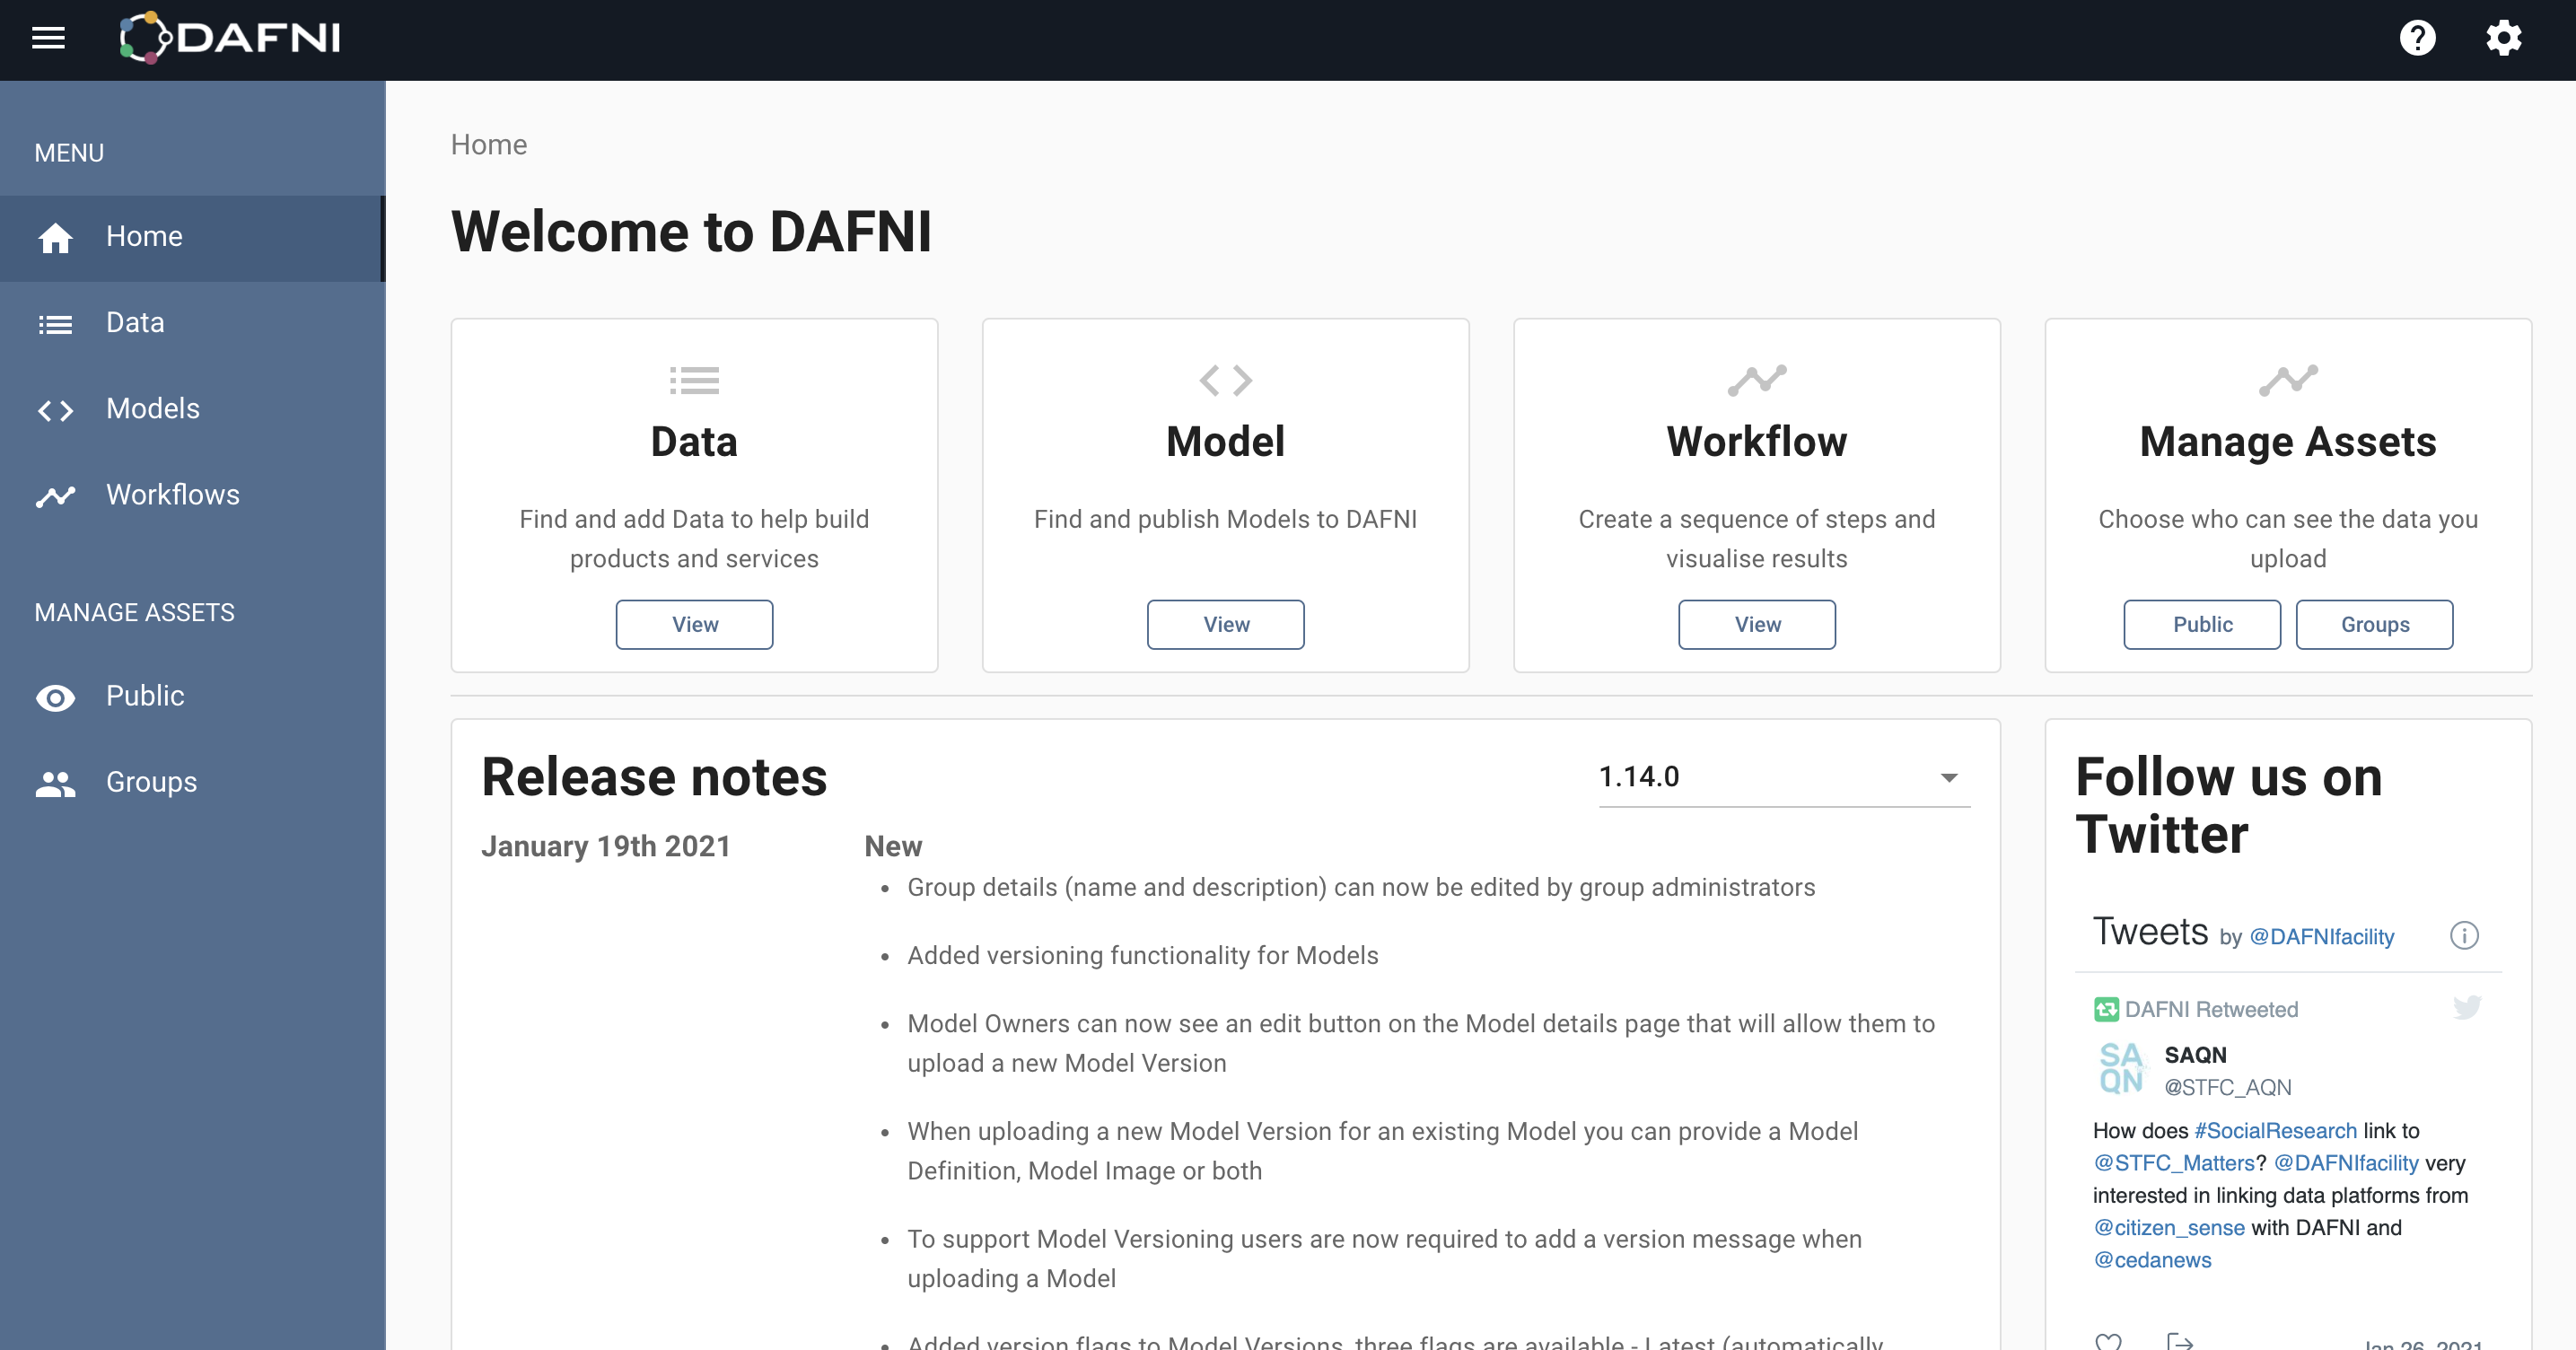
\includegraphics[width=0.8\linewidth]{figures/dafni-GUI.png}
\end{center}


}

\sframe{DAFNI workflow for coupled model}{

\centering

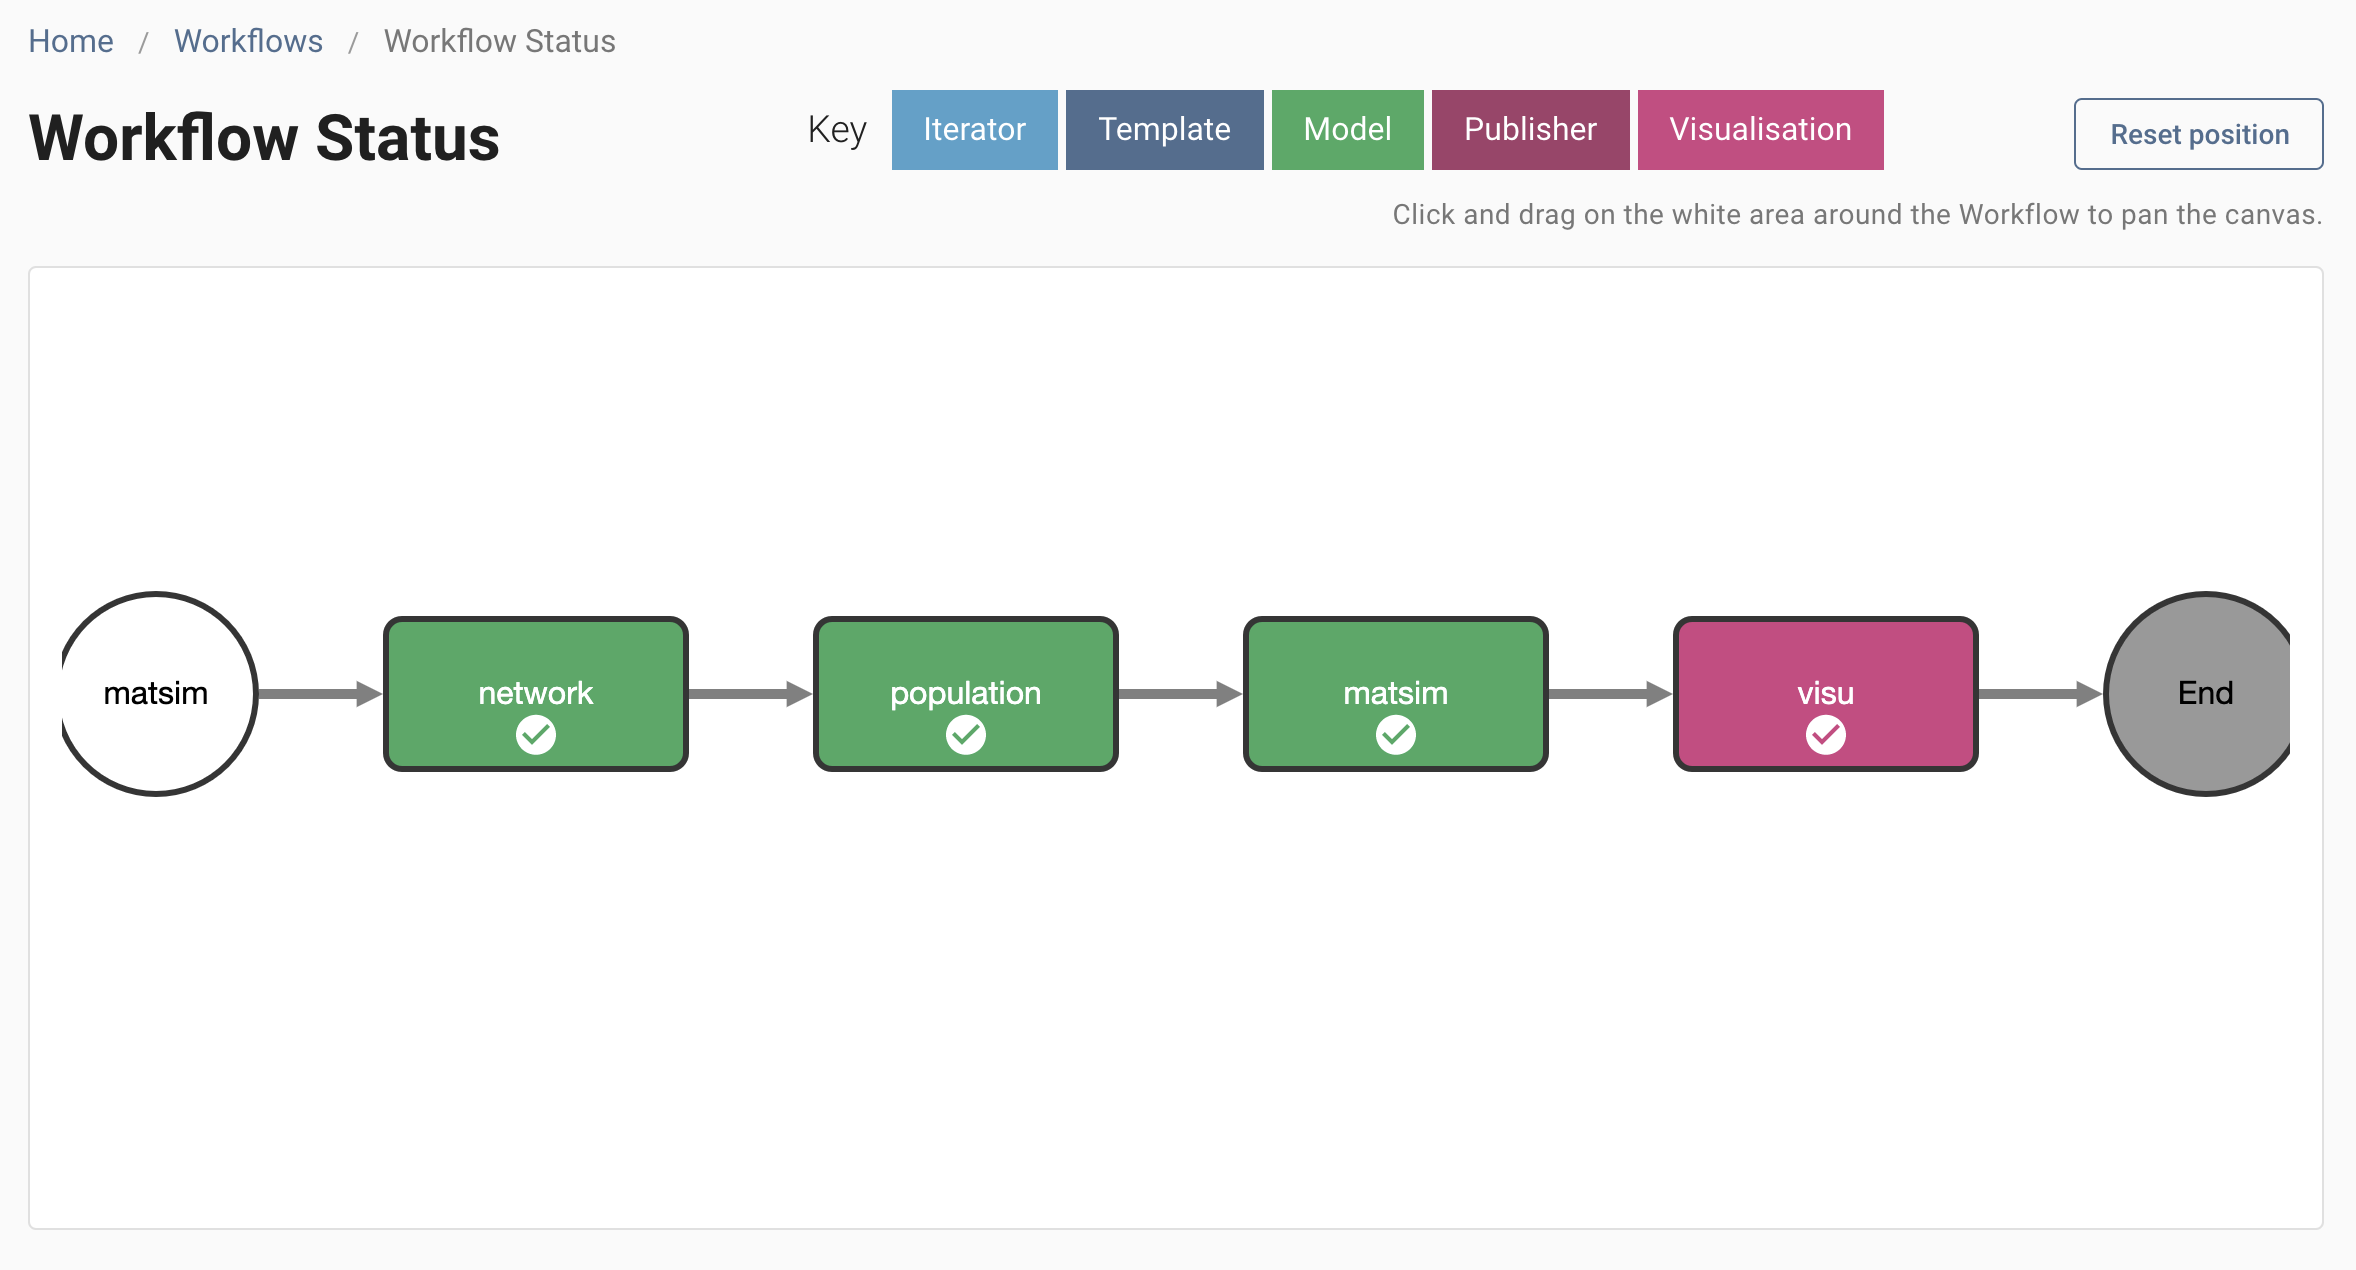
\includegraphics[width=\linewidth]{figures/matsim_workflow.png}

}

\sframe{Monte Carlo experiments}{

\centering

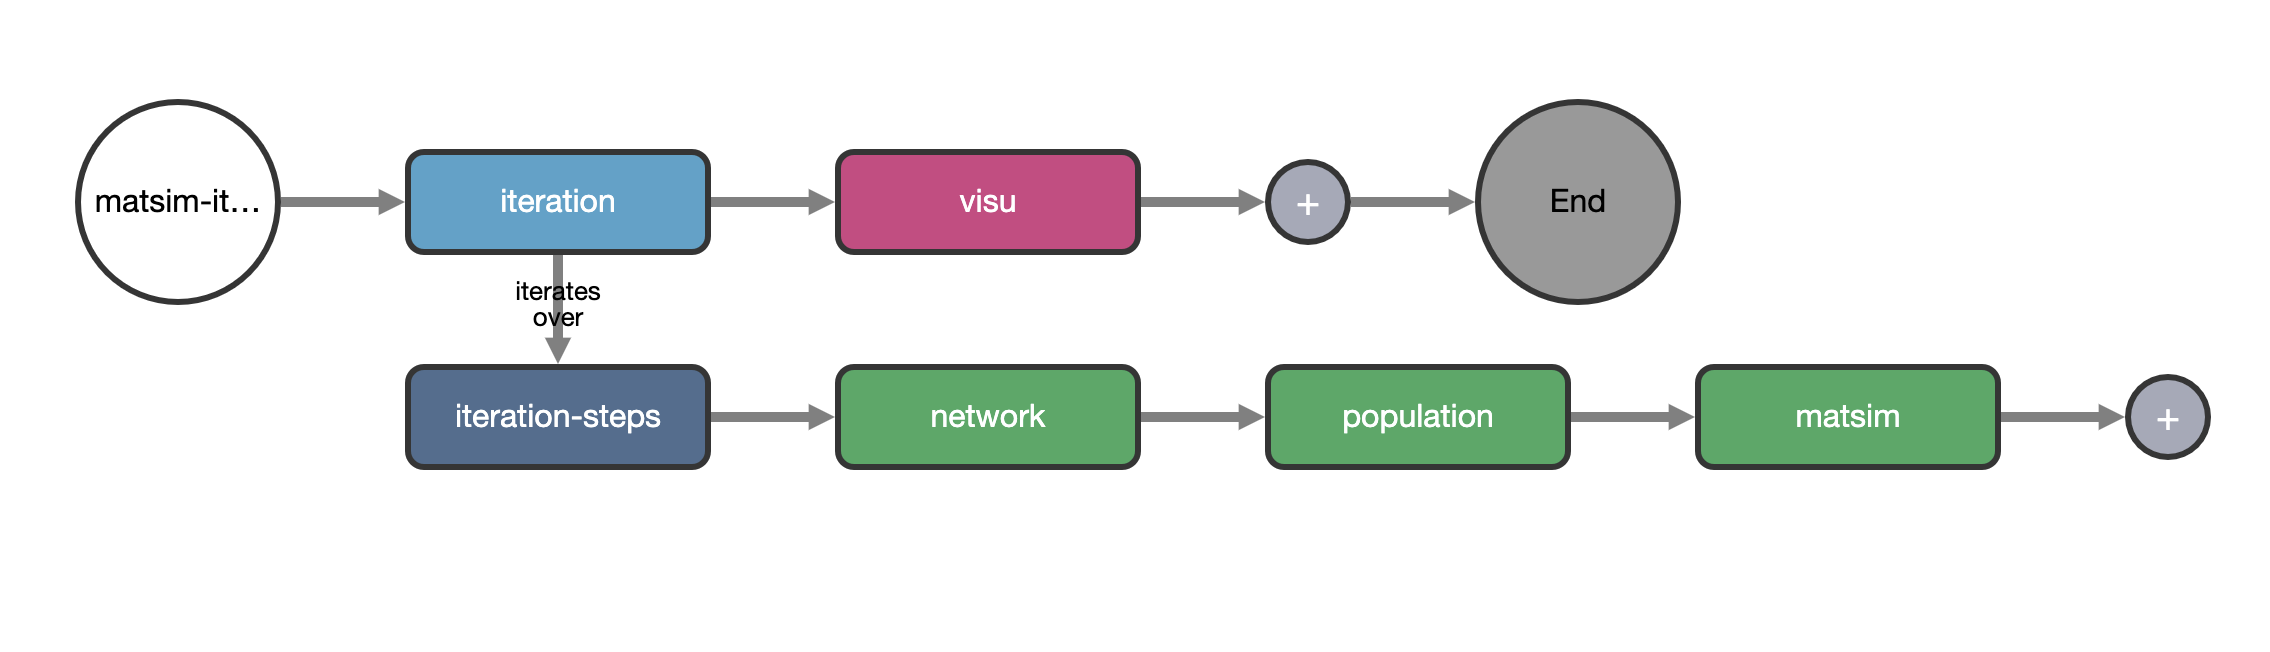
\includegraphics[width=\linewidth]{figures/matsim-iterations_workflow.png}

}

% The model is run on all functional urban areas in the UK. We show first results of numerical experiments comparing the use of the spatial interaction model with a null model to generate transport demand. We also study the role of stochasticity on model outputs, and show that spatial configuration has a significant influence.

\sframe{Visualization within DAFNI}{

\begin{center}
	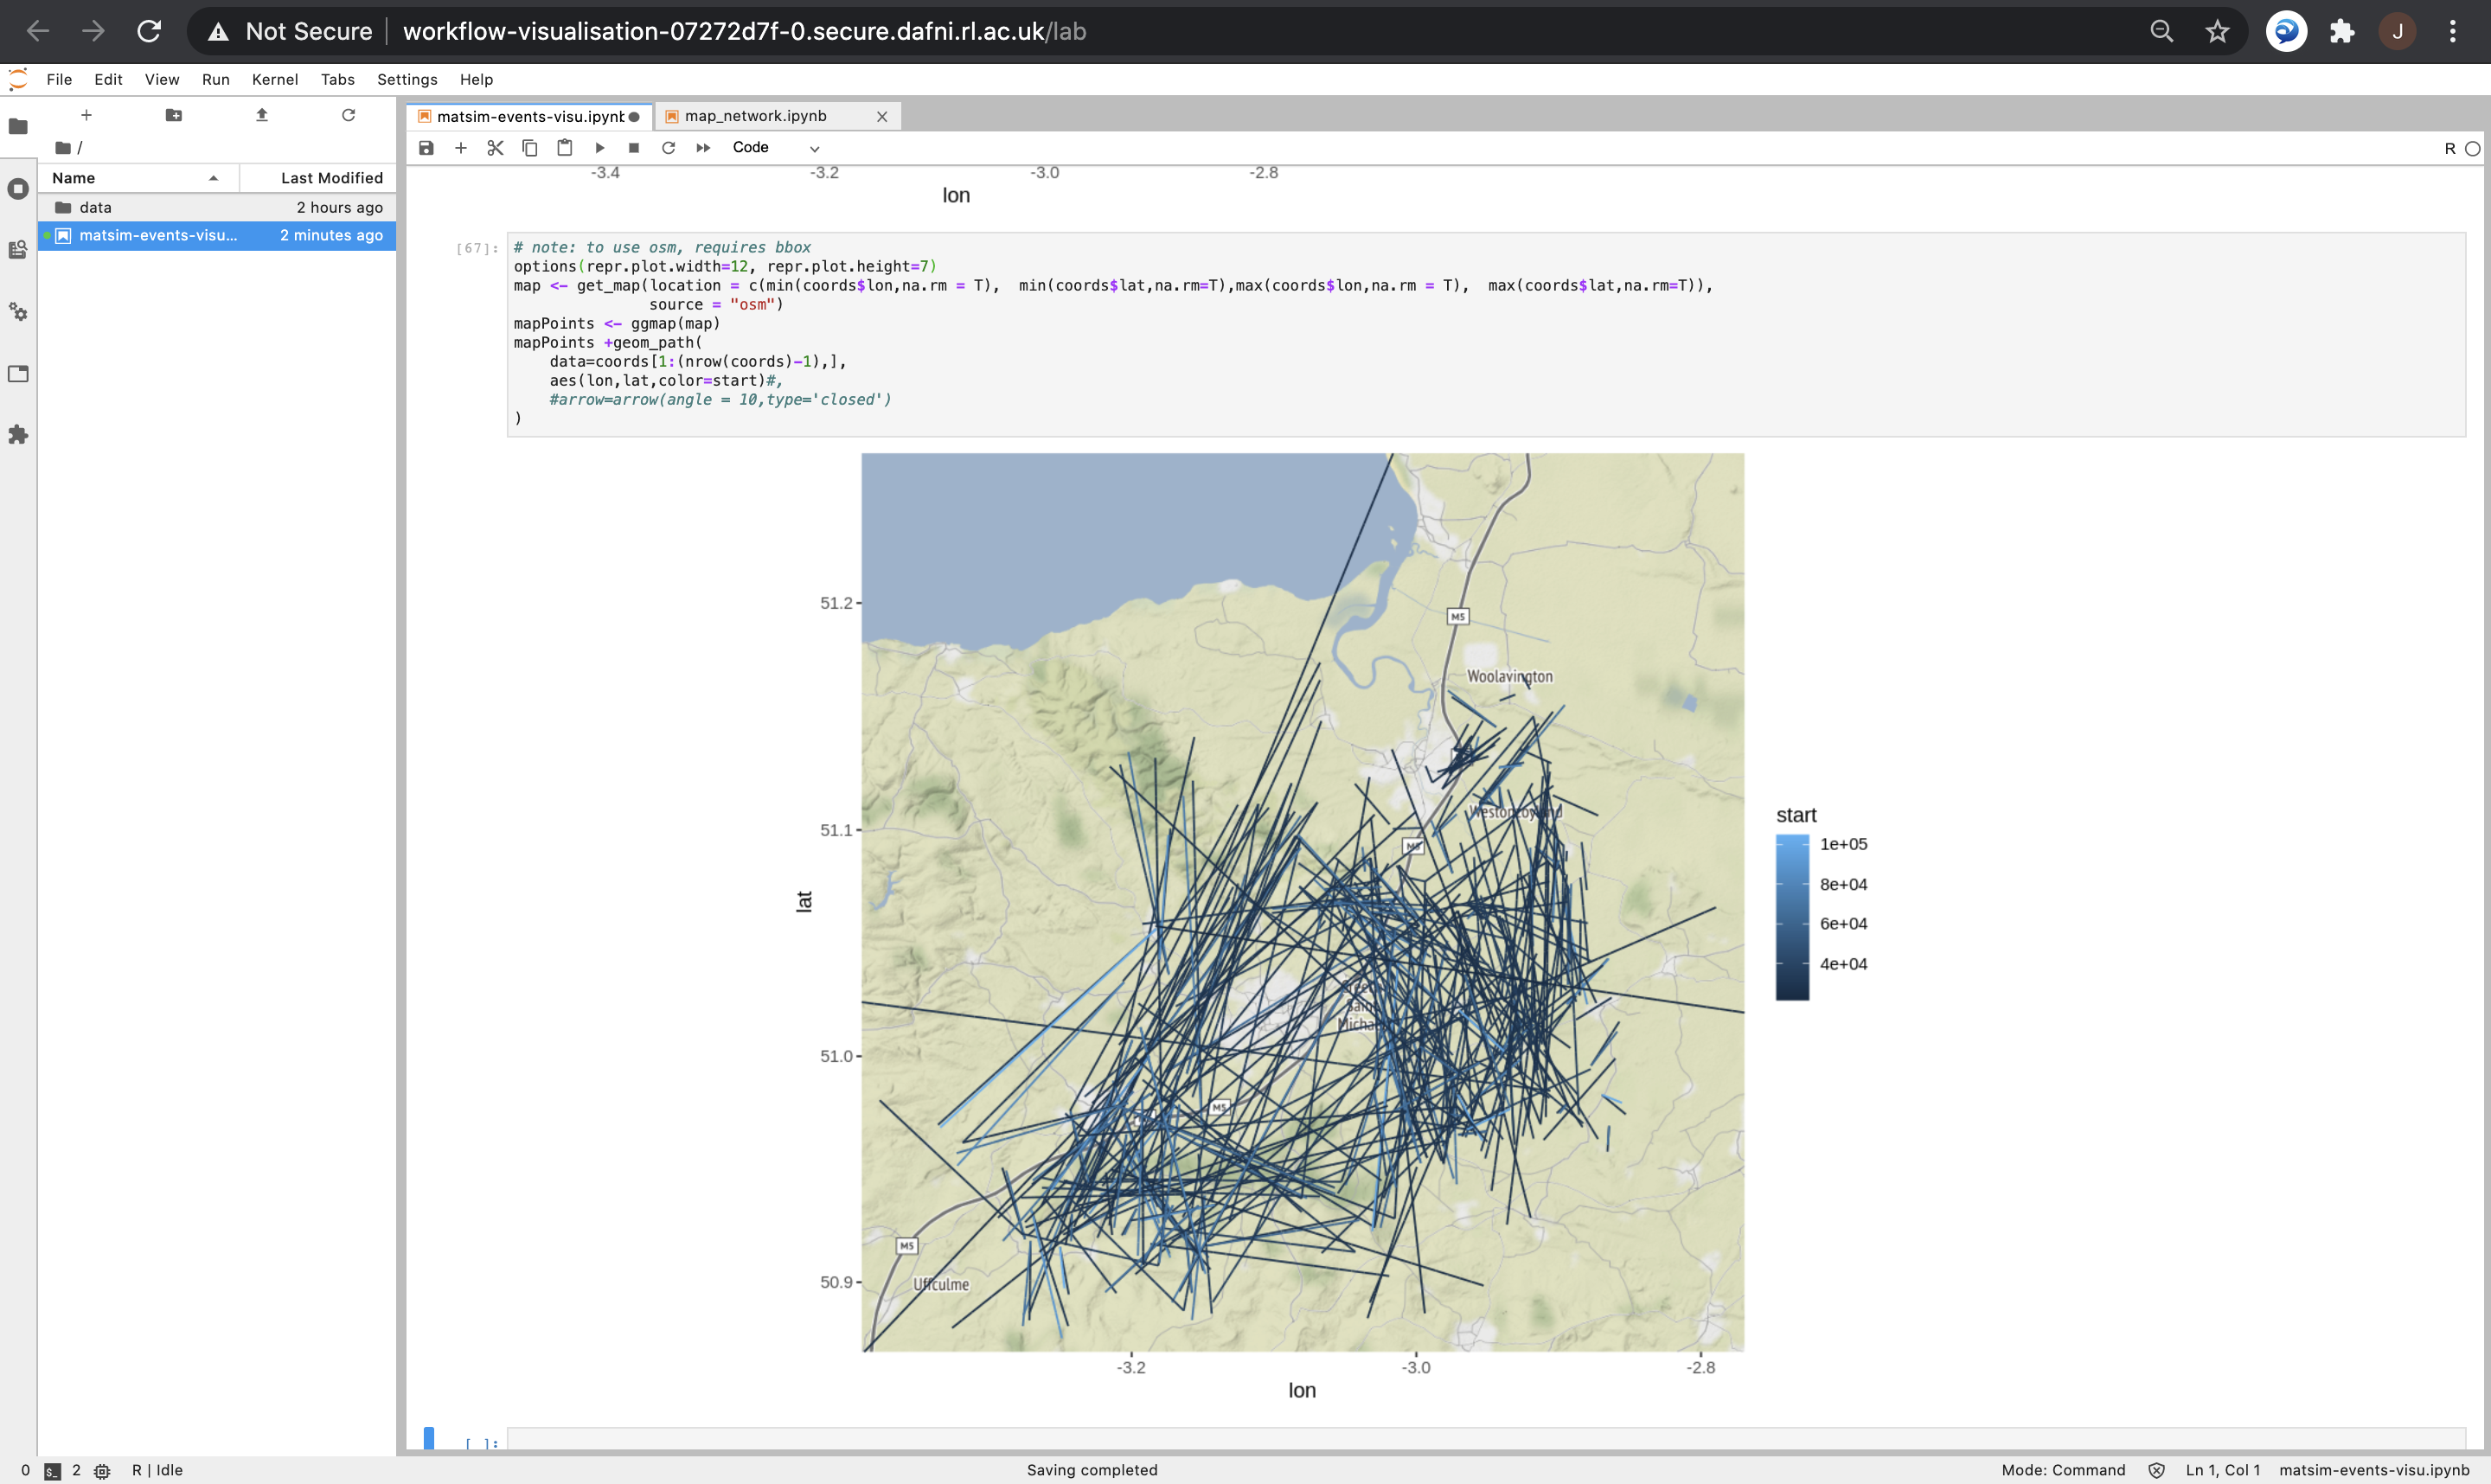
\includegraphics[width=\linewidth]{figures/visu_trips.png}	
\end{center}

}

\sframe{Visualization of trips: Leeds}{

\begin{center}
	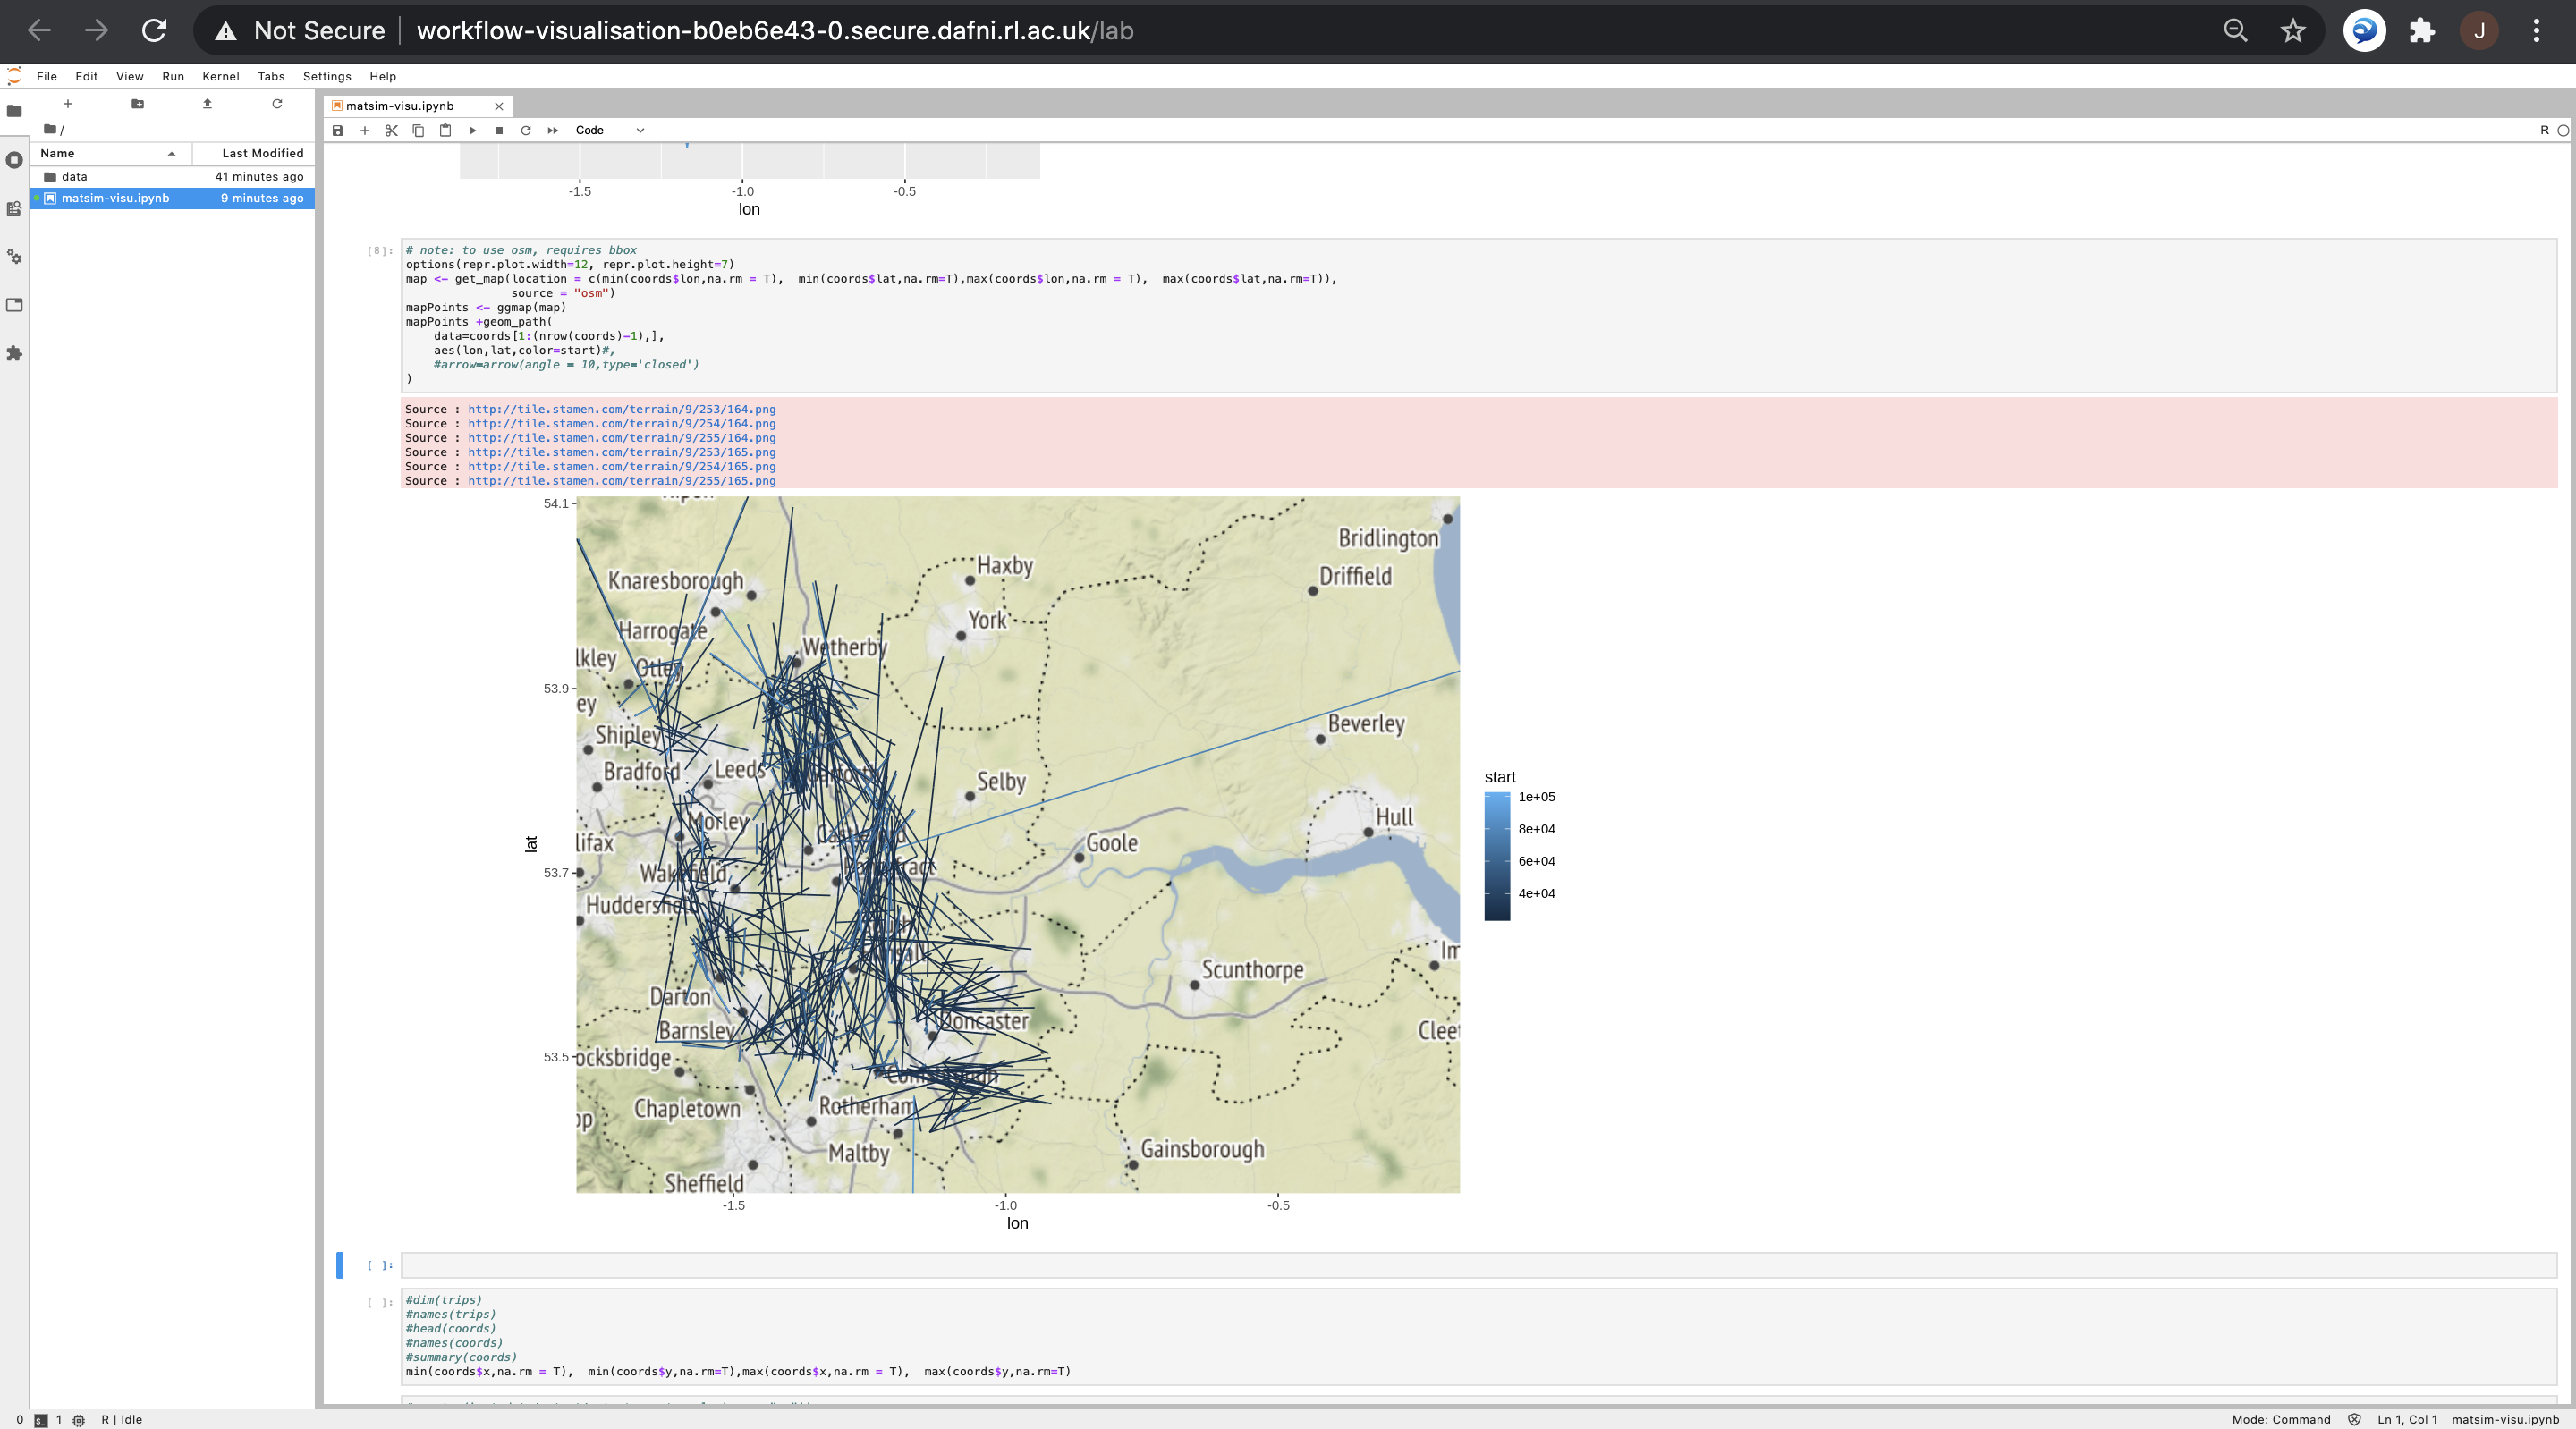
\includegraphics[width=\linewidth]{figures/visu-trips-Leeds.png}	
\end{center}

\medskip

\textit{Issue of sampling the synthetic population to decrease computation time}

}




\sframe{Simulation results: travel distances}{

% note: spatial interaction not implemented yet: simple synthetic pop
% discuss Matsim params? not needed - too complicated (reserve slide? not time! -> link to workflow)

\begin{center}
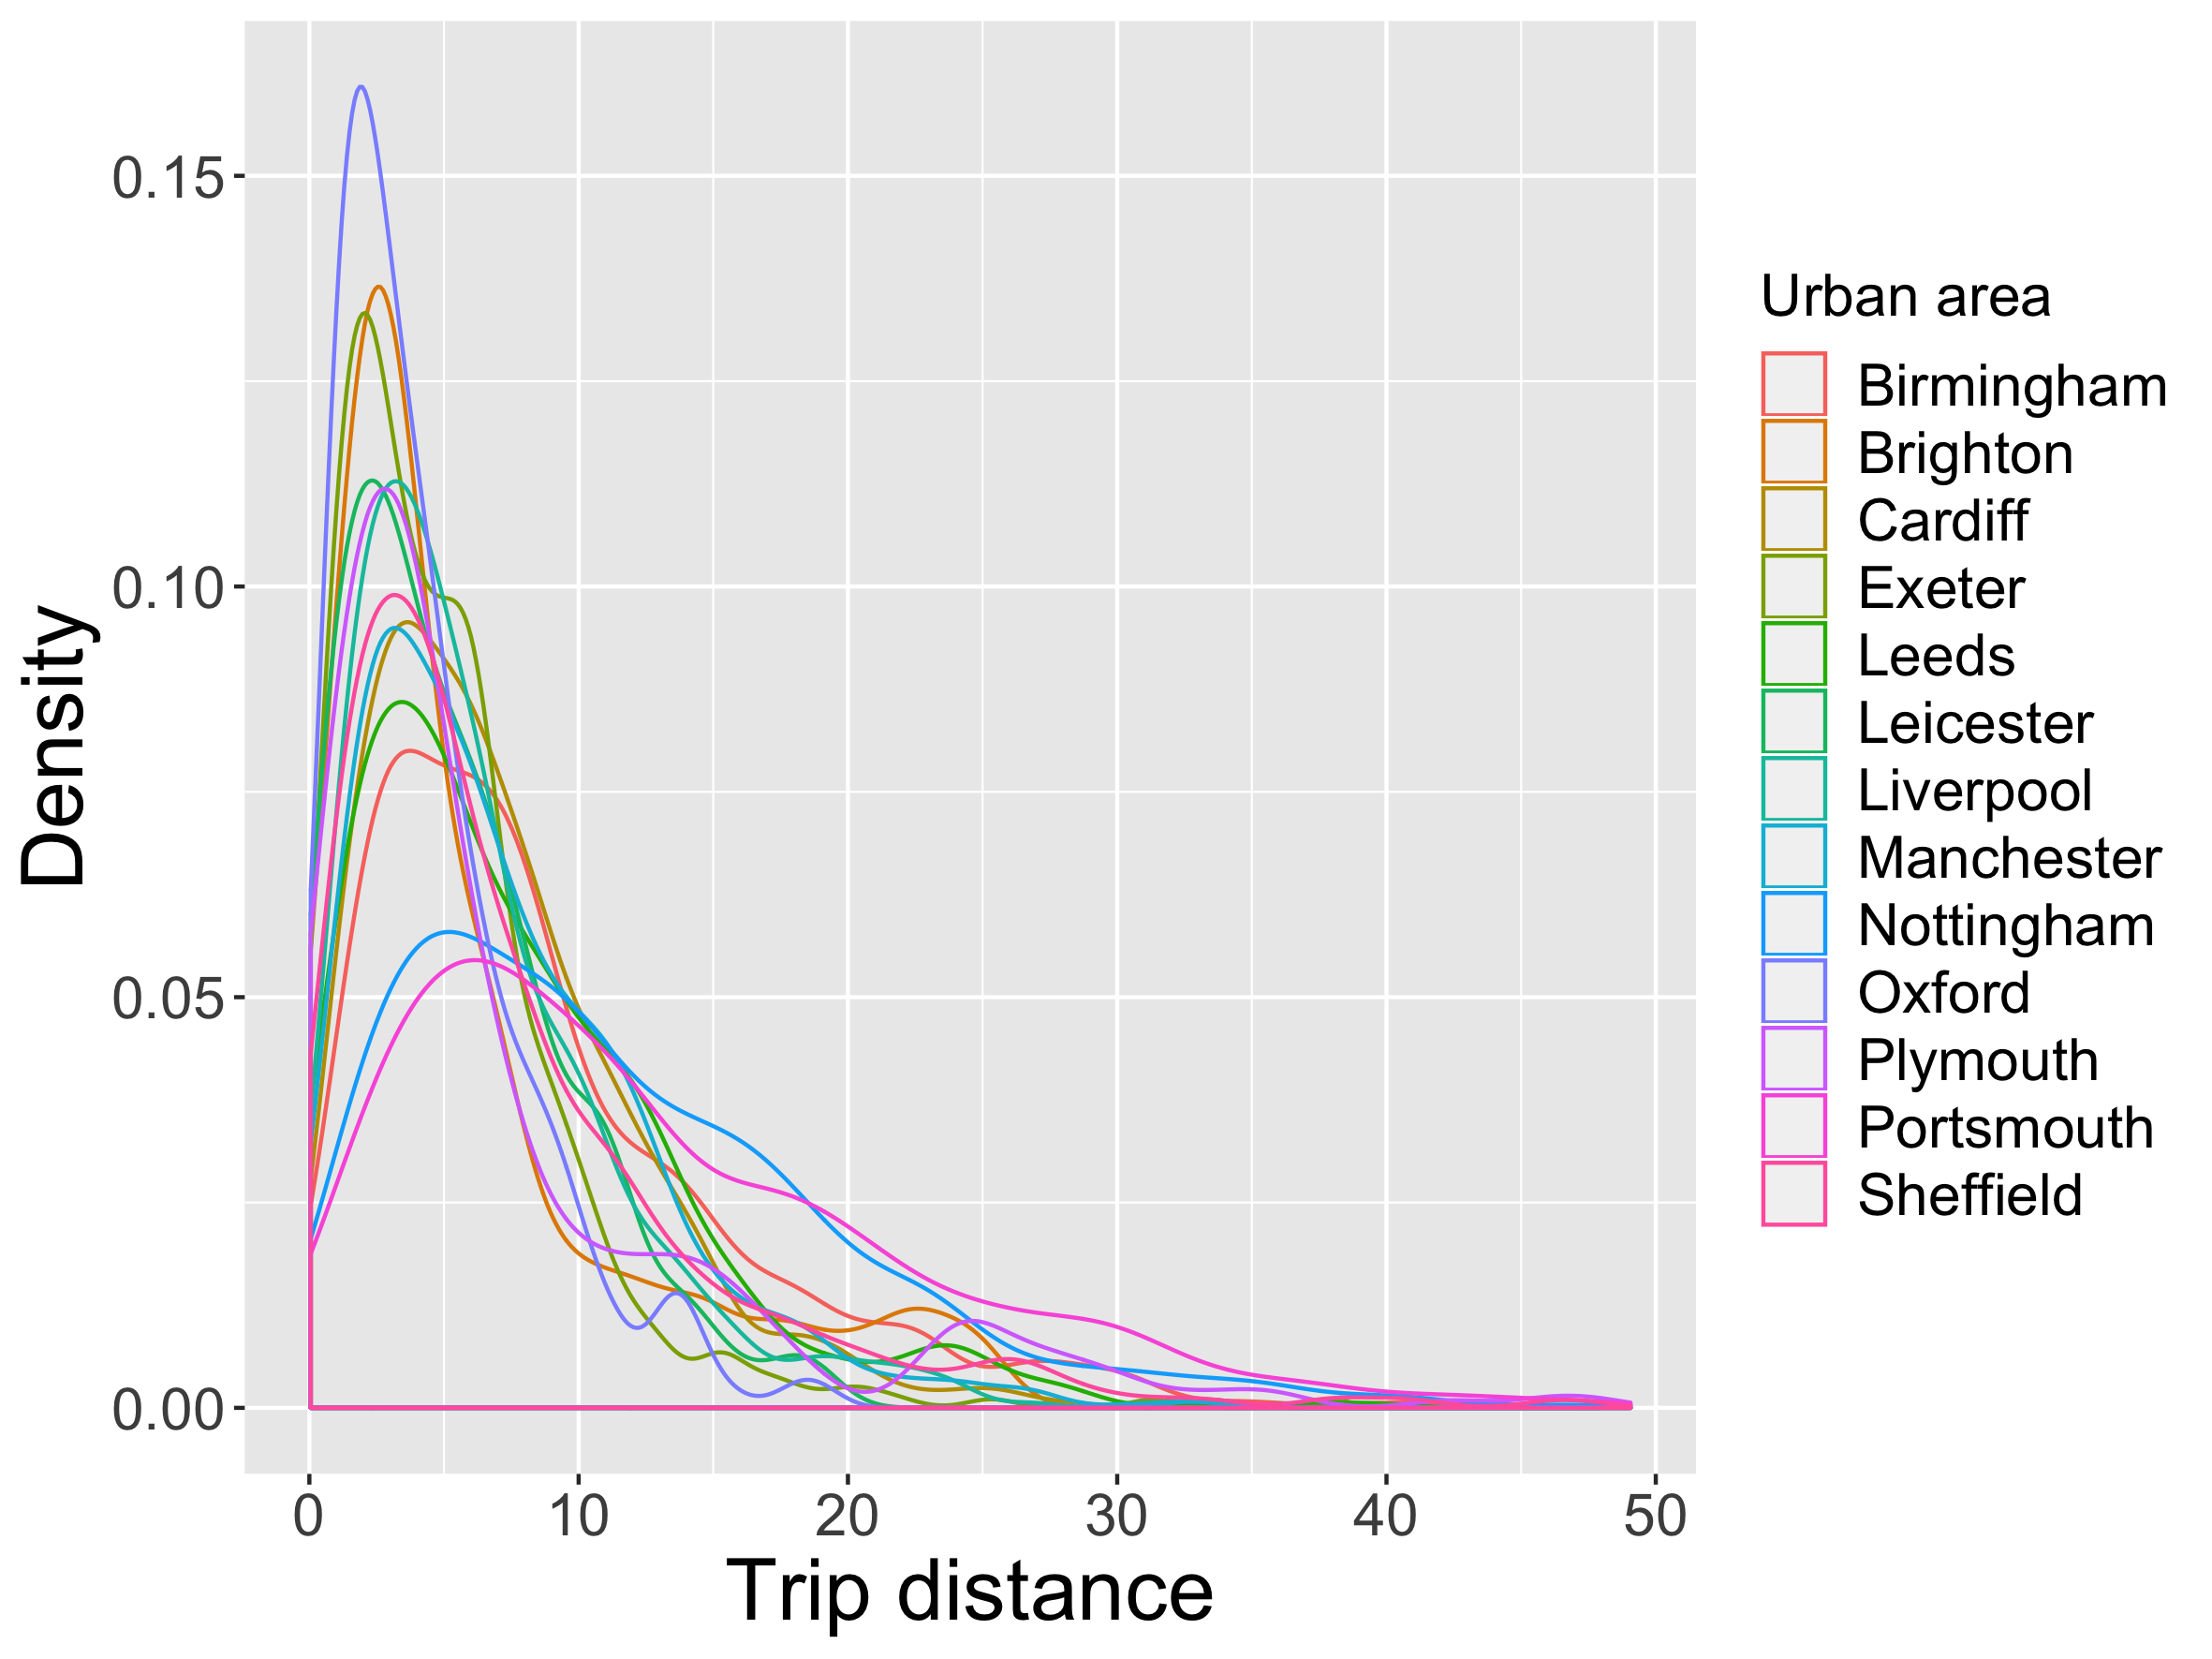
\includegraphics[width=\linewidth]{figures/distances_allFUAs.png}
\end{center}

}

\sframe{Daily travel patterns}{

departuretimes_allFUAs.png

}



\sframe{Role of stochasticity}{

\begin{center}
	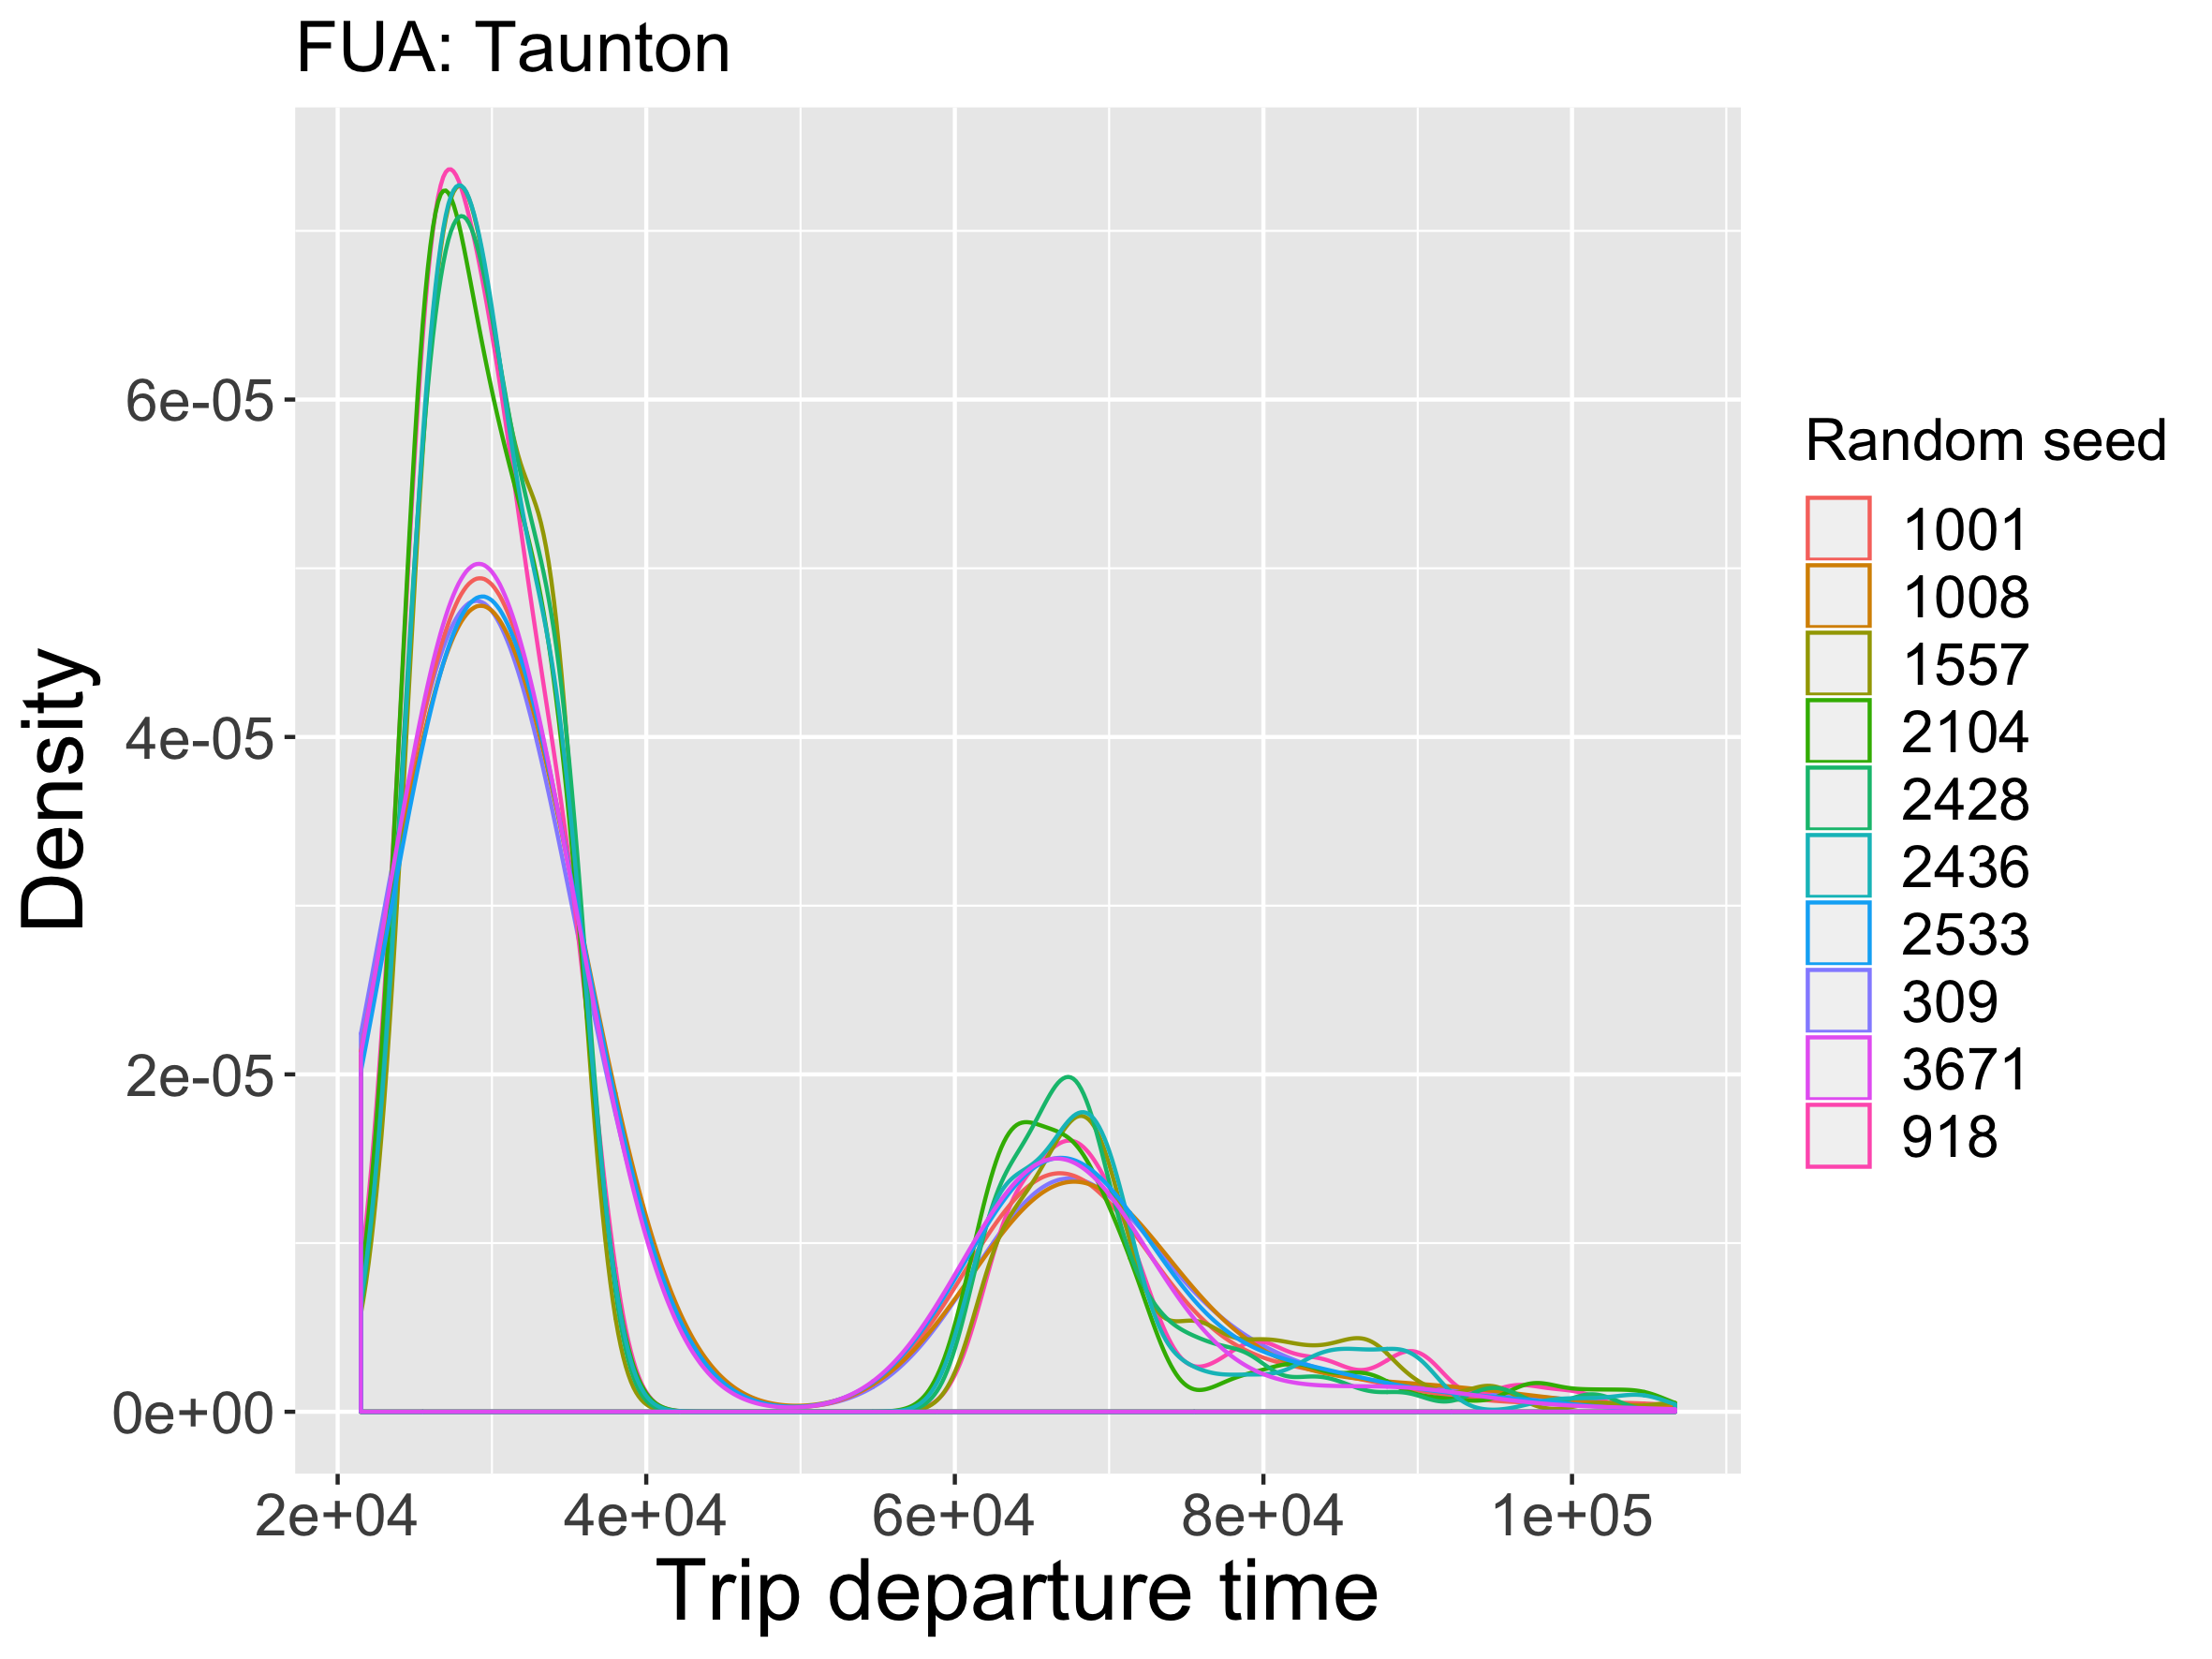
\includegraphics[width=0.9\linewidth]{figures/stochasticity_Taunton.png}	
\end{center}


}


\sframe{Validation: towards spatial sensitivity analysis}{

}





\section{OpenMOLE}

%To illustrate the reproducibility of our approach, we sketch the construction of the model with the OpenMOLE workflow engine, which provides a scripted workflow engine and methods to calibrate and validate simulation models, and suggest advanced numerical experiments for the validation of the coupled model.

\sframe{OpenMOLE workflow engine}{

}

\sframe{Coupling SPENSER and QUANT with OpenMOLE}{

\centering

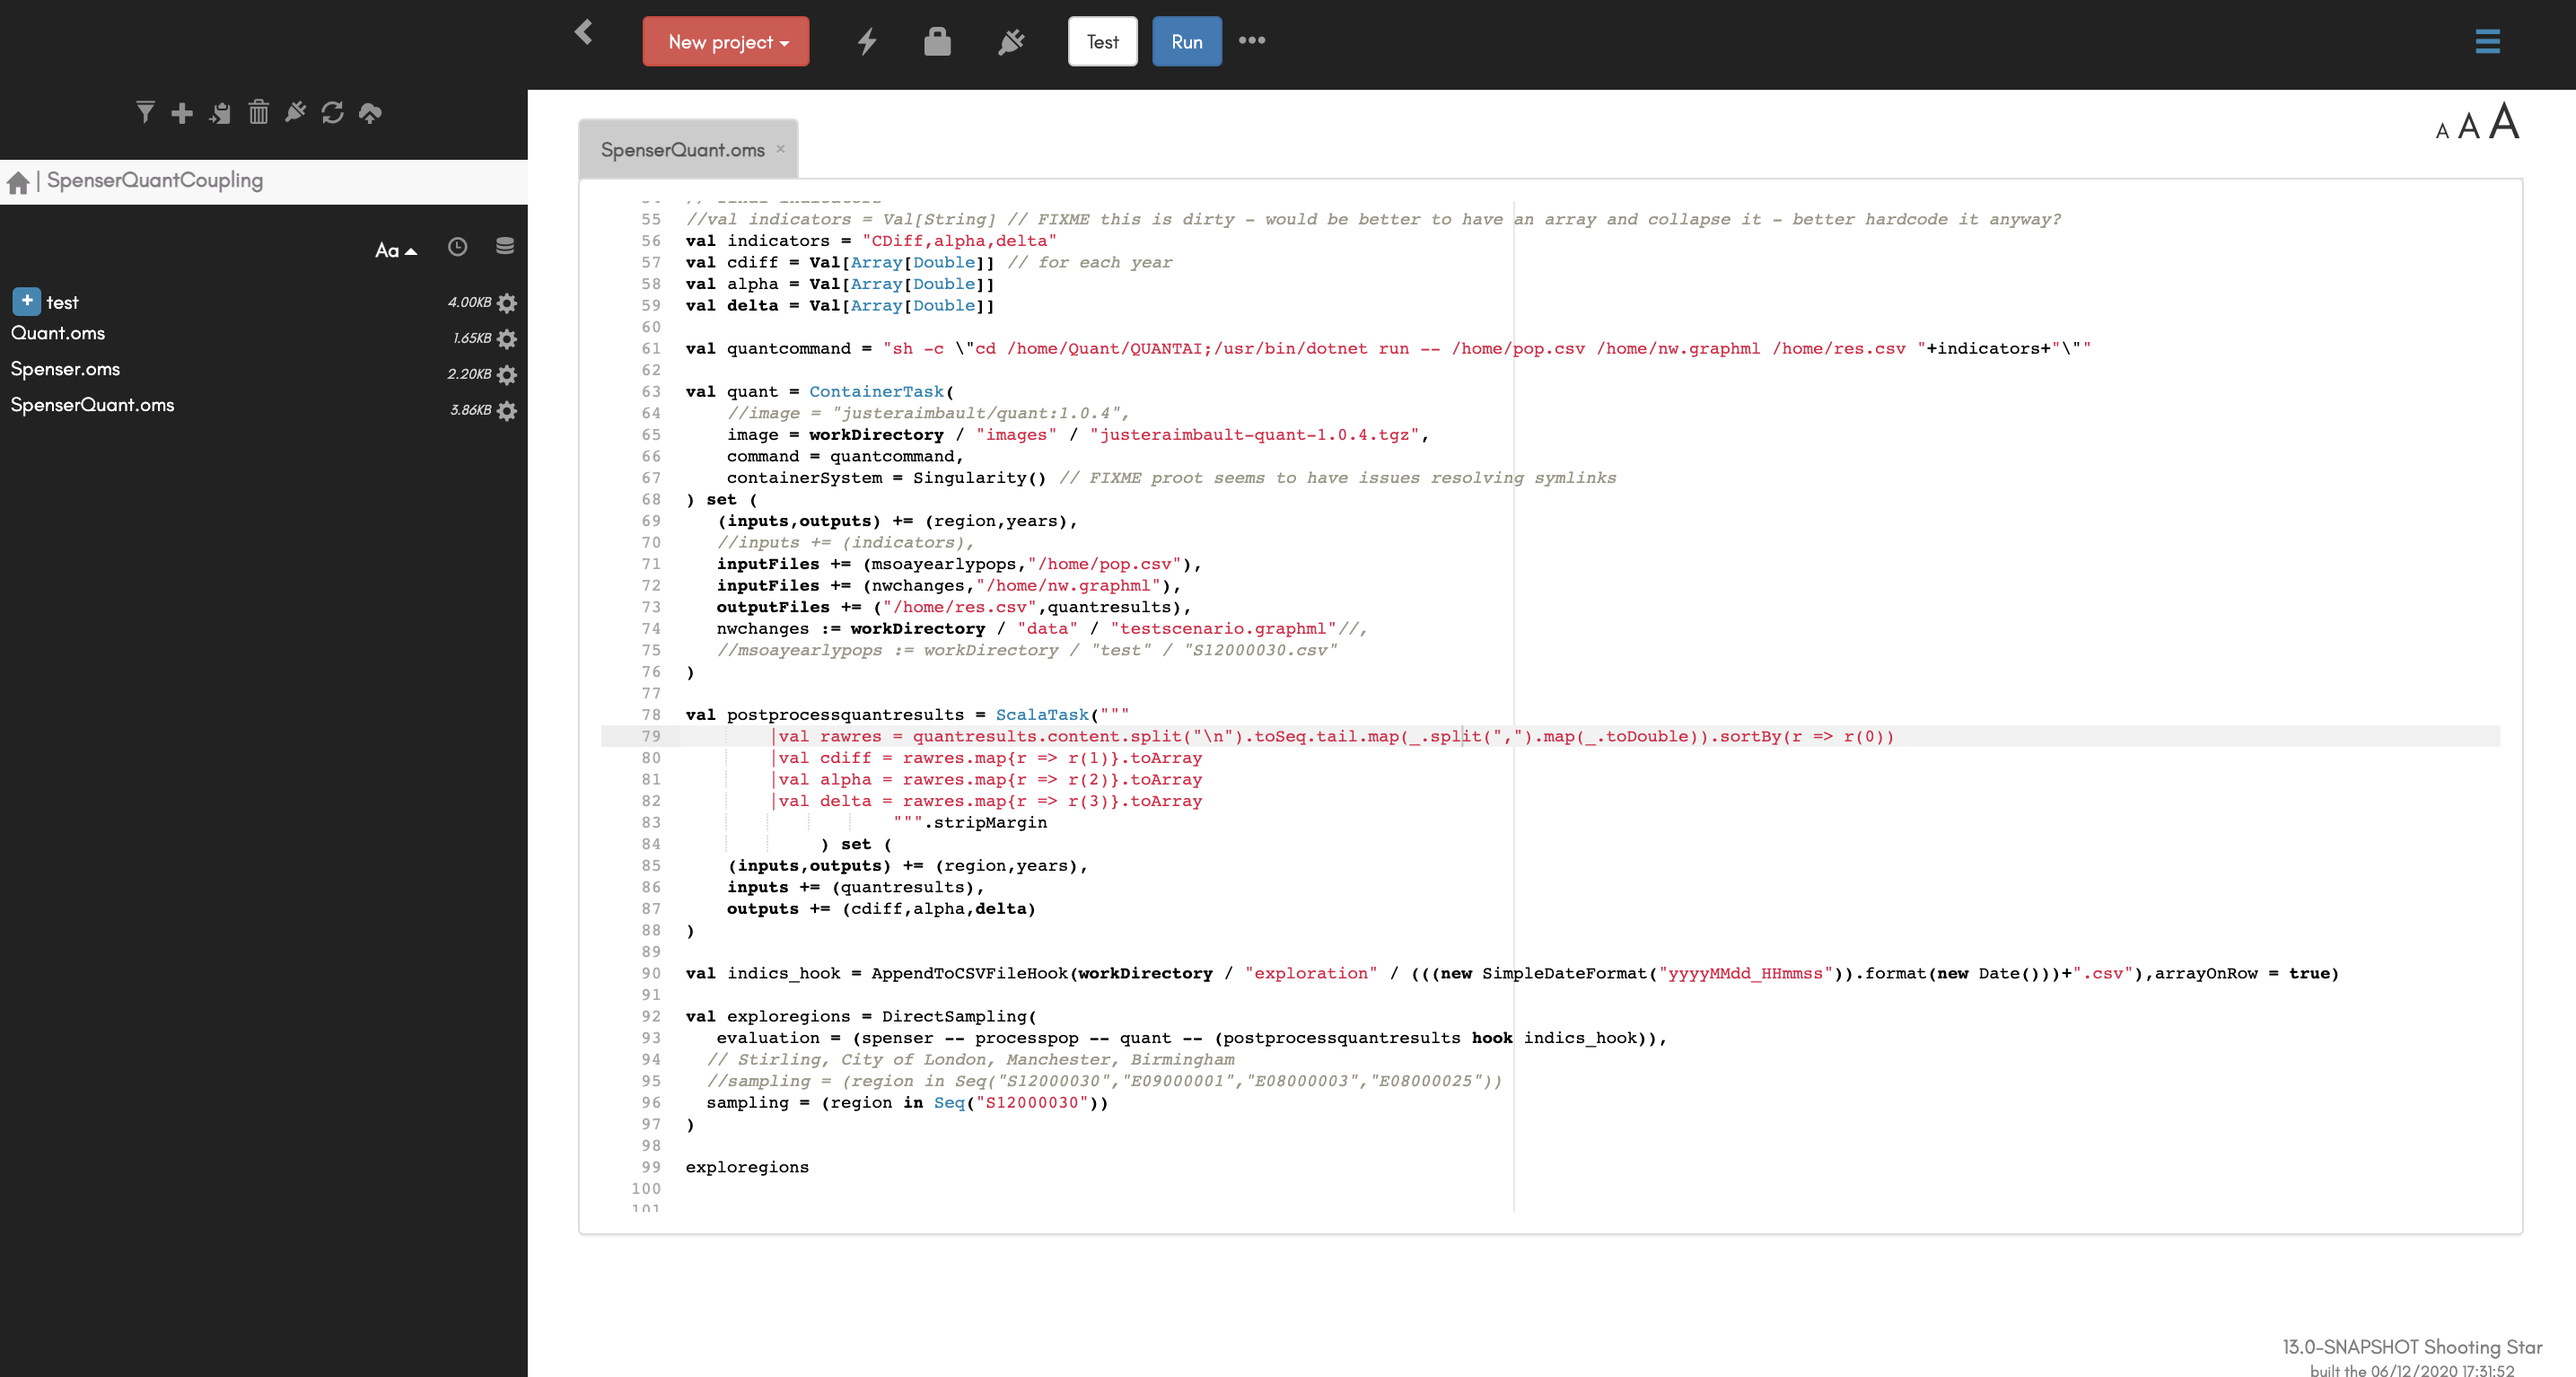
\includegraphics[width=\linewidth]{figures/openmole-spenserquant.png}

}

\sframe{Towards advanced validation experiments}{

}


\section{Discussion}

%We finally discuss ongoing developments on the application of this model to the development of health indicators within public transportation, and more particularly linking transportation and work-from-home policies with effective densities in public transport which provide potential exposure indicators in the context of the COVID-19 crisis.

\sframe{Discussion}{

}



\sframe{Conclusion}{


$\rightarrow$ 


\bigskip
\bigskip

\textbf{Open repositories}

\url{https://github.com/JusteRaimbault/UrbanDynamics} for workflows


\bigskip

\textbf{Workflow engines}

}



%%%%%%%%%%%%%%%%%%%%%
\begin{frame}[allowframebreaks]
\frametitle{References}
\bibliographystyle{apalike}
\bibliography{biblio}
\end{frame}
%%%%%%%%%%%%%%%%%%%%%%%%%%%%


%
%\sframe{Reserve slides}{
%
%\Huge
%
%\centering
%
%Reserve slides
%
%% possible questions?
%% application to real systems?
%% policy applications?
%% def/carac coevol
%% multiscale? ~
%
%}
%
%
%\sframe{Defining co-evolution}{
%
%}
%
%\sframe{Characterizing co-evolution}{
%
%}
%
%\sframe{A LUTI model with governance processes}{
%
%}




\end{document}

